\documentclass[12pt, a4paper]{article}
\usepackage[utf8]{inputenc}
\usepackage{amsmath}
\usepackage{graphicx}
\usepackage{fancyhdr}
\usepackage{geometry}
\usepackage{fixltx2e}
\usepackage{amsfonts}
\usepackage{multicol}
\usepackage{amssymb}
\usepackage{tabto}

\geometry{margin=1.2in}




\def\separator{\begin{center}    \rule{100pt}{0.5pt}\end{center}}

\setlength{\parindent}{0em}
\setlength{\parskip}{1em}

\geometry{margin=1.2in}




\def\separator{\begin{center}    \rule{100pt}{0.5pt}\end{center}}

\setlength{\parindent}{0em}
\setlength{\parskip}{1em}

\begin{document}
\section{prime lezioni}
insiemi e logica elementare

numeri reali e naturali

\section{maggioranti, minoranti, sup e inf}

\textbf{Def}\\ Sia $A\in\mathbb{R}$ non vuoto.\\ $A$ è \textbf{limitato superiormente} se esiste $M\in\mathbb{R}$
tale che $x\leq M$ $\forall x\in A$. $M$ viene definito come \textbf{Maggiorante} di $A$. Se $M$ di $A$ appartiene
ad $A$ si dice \textbf{massimo} di $A$, e viene denotato come $max(A)$

$A$ è \textbf{limitato inferiormente} se esiste $m\in\mathbb{R}$ tale che $x\geq M$ $\forall x\in A$. $m$ viene
definito come \textbf{minorante} di $A$. Se $m$ di $A$ appartiene ad $A$ si dice \textbf{minimo} di $A$, e viene
denotato come $min(A)$

$A$ si dice \textbf{limitato} se è limitato sia inferiormente che superiormente

\textbf{Def}\\ Siano $A,B\in\mathbb{R}$ non vuoti
\begin{itemize}
    \item $-A \doteq \{-x \mid x\in A\}$
    \item $A+B \doteq \{x+y\mid x\in A,\ y\in B\}$
    \item $A-B \doteq \{x-y\mid x\in A,\ y\in B\}$
\end{itemize}
Se $x\in\mathbb{R}$
\begin{itemize}
    \item $x+A\doteq\{x+y\mid y\in A\}$
\end{itemize}

non importante, skippo

\section{lezioni skippate}
Caratterizzazione sup, inf, classi contigue, densità dei razionali

\section{Radici, esponenziali reali, funzioni inverse, logaritmi, trigonometriche}

\textbf{Prop - Radici n-esima}\\
per ogni numero nullo positivo $a$ e per ogni $n\in\mathbb{N}$ esiste un unico numero reale $b$ tale
che $b^{n}=a$. Tale reale positivo è la radice n-esima e si indica con i simboli:
\begin{center}
    $\sqrt[n]{a}\quad\doteq\quad a^{\frac{1}{n}} $
\end{center}

Sia $r\in\mathbb{Q},  r=\frac{p}{q},  p\in\mathbb{Z}  q\in\mathbb{N}$. Allora se $a>0$:
\begin{center}
    $a^{r}\doteq a^{\frac{p}{q}}\doteq \sqrt[q]{a^{p}} \qquad r\geq 0$

    $a^{r}\doteq a^{\frac{p}{q}}\doteq \frac{1}{\sqrt[q]{a^{-p}}} \qquad r<0$
\end{center}

La radice possiede le stesse proprietà della potenza intera

Se $0<a<1$, allora posto $b=\frac{1}{a}$ e definisco:
\begin{center}
    $a^{x}=\frac{1}{b^{x}}$
\end{center}

\textbf{Operazioni tra funzioni}\\$f,g$
    \begin{itemize}
        \item Somma: $(f+g)(x)\doteq f(x)+g(x)\qquad x\in dom(f)\cap dom(g)\neq \emptyset$
        \item Prodotto: $(f\times g)(x)\doteq f(x)\times g(x)\qquad x\in dom(f)\cap dom(g)\neq \emptyset$
        \item Rapporto: $(\frac{f}{g})(x)\doteq \frac{f(x)}{g(x)}\qquad x\in dom(f)\cap dom(g)\neq \emptyset
                  , g(x)\neq 0$
        \item Composizione: $(f\circ g)(x)\doteq f(g(x))\qquad \forall x\in A$
        \item Restrizione: $f:A\rightarrow\mathbb{R}\quad A\subseteq\mathbb{R},  A\neq\emptyset$. Se prendo
              $B\subseteq A$ allora la resitrzione $AB$ di $f$ è: $f\upharpoonright_{B}:  B\rightarrow\mathbb{R}$
    \end{itemize}

    \textbf{Def - funzioni limitate}\\ Sia $f:A\rightarrow\mathbb{R},  A\subseteq\mathbb{R}  A\neq\emptyset$,
    diremo che $f$ è \textbf{limitata superiormente} se $f(A)\subseteq\mathbb{R}$ è limitata superiormente,
    cioé esiste $M\in\mathbb{R}$ tale che $f(x)\leq M\quad \forall x\in A$. Analogamente diremo che $f$ è
    \textbf{limitata inferiormente} se $f(A)\subseteq\mathbb{R}$ è limitata inferiormente, cioé esiste
$m\in\mathbb{R}$ tale che $f(x)\geq m\quad \forall x\in A$.\\La funzione $f$ sarà \textbf{limitata} se
    è limitata inferiormente e superiormente.

    Quindi se $f(A)$ è limitata superiormente allora esiste il suo estremo superiore $sup(f(A))$, ovvero
$sup(f)\doteq sup(f(A))$. Lo stesso vale per l'opposto ($inf(f)\doteq sup(f(A))$).\\ Se $x_{0}\in dom(A)$
    e $f(x_{0})=sup(f)$ si dice che $f$ ammette \textbf{massimo assoluto}. Nel caso dell'estremo inferiore,
    diremo che $f$ ammette \textbf{minimo assoluto}

    \textbf{Def - funzioni monotone}\\Sia $f:A\rightarrow\mathbb{R},  A\subseteq\mathbb{R}  A\neq\emptyset$.
    Allora $f$ è detta:
    \begin{itemize}
        \item Crescente: per ogni coppia $x_{1},x_{2}\in A$, se $x_{1}<x_{2}\Rightarrow f(x_{1})\leq f(x{_2})$
        \item Strettamente crescente: per ogni coppia $x_{1},x_{2}\in A$, se $x_{1}<x_{2}\Rightarrow f(x_{1})<f(x{_2})$
        \item Decrescente: per ogni coppia $x_{1},x_{2}\in A$, se $x_{1}<x_{2}\Rightarrow f(x_{1})\geq f(x{_2})$
        \item Strettamente Decrescente: per ogni coppia $x_{1},x_{2}\in A$, se $x_{1}<x_{2}\Rightarrow f(x_{1})>f(x{_2})$
    \end{itemize}
    Le funzioni crescenti e decrescenti vengono definite monotone, mentre quelle strettamente crescenti o decrescenti
    sono strettamente monotone

    \textbf{Prop}\\Ogni funzione strettamente monotona è iniettiva

    Osservazioni:\\se $f$ è iniettiva, non per forza è strettamente monotona, ma vale la negazione: se una funzione
    non è iniettiva, allora sicuramente non è strettamente monotona.

    \textbf{Def - Funzioni inverse}\\Sia $A\subseteq\mathbb{R}$ non vuoto e $f:A\rightarrow B$. Se $f$ è biunivoca
    (iniettiva e suriettiva) allora $f$ è \textbf{invertibile} e si chiama funzione inversa di $f$ la funzione
$g:B\rightarrow A$ e vale:
    \begin{center}
        $\qquad g\circ f= id(A)\qquad (id(x)=x\quad \forall x\in A)$
    \end{center}
    La funzione inversa si indica con il simbolo $f^{-1}$

    \textbf{Def - Funzioni periodiche}\\Sia $f:\mathbb{R}\rightarrow\mathbb{R}$. Si dice che $f$ è \textbf{periodica}
    se esiste $t\in\mathbb{R}/\{0\}$ tale che:
    \begin{center}
        $f(x+t)=f(x)\qquad \forall x\in\mathbb{R}$
    \end{center}
$t$ è detto periodo di $f$. Il numero $t_{0}\doteq min\{t>0\}$ è detto, se esiste, \textbf{minimo periodo} di $f$

    \textbf{Def - Polinomi e razionali}
    \begin{center}
        $P(x) = a_{0}+a_{1}x+a_{2}x^{2}+...+a_{n}+x^{n} \qquad a_{0},...a_{n}\in\mathbb{R},  n\in\mathbb{N}$
    \end{center}
    Se $a_{n}\neq 0$ allora diremo che $n$ è il grado del polinomio. $P$ è definito su tutto $\mathbb{R}$.
    I valori $x\in\mathbb{R}$ per cui $P(x)=0$ sono detti zeri o radici. Se $P$ ha grado $n$, allora le radici sono
    al più $n$ numeri reali.\\$P$ è detto \textbf{irriducibile} se non è scrivibile come prodotto di polinomi di grado
minore al grado di $P$. Gli unici polinomi a essere irriducibili sono quelli di 1° grado e quelli di 2° grado con
discriminante negativo

Una funzione $f$ è \textbf{razionele} se:
\begin{center}
    $f(x)=\frac{n(x)}{d(x)}$
\end{center}
dove $n(x)$ e $d(x)$ polinomi, $dom(f)=\{x\in\mathbb{R}\mid d(x)\neq 0\}$.\\Se $f$ è razionale e $grad(n)>grad(d)$
allora:
\begin{center}
    $f(x)=P(X)+\frac{r(x)}{d(x)}$
\end{center}
dove $P(x)$ è polinomio quoziente e $r(x)$ è il resto della divisione

\textbf{Funzioni trigonometriche e le loro inverse}
\begin{center}
    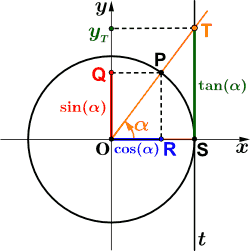
\includegraphics[width=150px]{images/trigon.png}\\
    $cos(x)=sin(x+\frac{\pi}{2})$\\
    $cos(x)^{2}+sin(x)^{2}=1$
\end{center}
parità: coseno è pari, infatti $cos(-x)=cos(x)$, mentre il seno è dispari perché $sin(-x)=-sin(x)$

\textbf{tangente e cotangente}\\la tangente, $tg(x)=\frac{sin(x)}{cos(x)}$, corrisponde alla lunghezza del segmento
che cade perpendicolare sull'asse delle x nel punto 1 e che interseca l'estensione del raggio. Il dominio della
tangente è $dom(tg)=\mathbb{R}/\{x=\frac{\pi}{2}+k\pi\mid k\in\mathbb{Z}\}$. La contangente,
$tg(x)=\frac{cos(x)}{sin(x)}$, invece cade sull'asse delle y nel punto 1.

Sia tangente e cotangente sono funzioni dispari e hanno periodo minimo in $\pi$

\textbf{Inverse}
\begin{center}
    $arcsin:[-1,1]\rightarrow[-\frac{\pi}{2},\frac{\pi}{2}]$\\
    $arcsin\doteq(sin\upharpoonright_{[-\frac{\pi}{2},\frac{\pi}{2}]})^{-1}$\\
    $arcsin(sin(x))=x \qquad \forall x\in[-\frac{\pi}{2},\frac{\pi}{2}]]$
\end{center}

\begin{center}
    $arccos:[-1,1]\rightarrow[0,\pi]$\\
    $arccos\doteq(cos\upharpoonright_{[0,\pi]})^{-1}$\\
    $arccos(cos(x))=x \qquad \forall x\in[0,\pi]$
\end{center}

\begin{center}
    $arctg:[-1,1]\rightarrow[-\frac{\pi}{2},\frac{\pi}{2}]$\\
    $arctg\doteq(tg\upharpoonright_{[-\frac{\pi}{2},\frac{\pi}{2}]})^{-1}$\\
    $arctg(tg(x))=x \qquad \forall x\in[-\frac{\pi}{2},\frac{\pi}{2}]]$
\end{center}

\begin{center}
    $arccotg:[-1,1]\rightarrow[0,\pi]$\\
    $arccotg\doteq(cotg\upharpoonright_{[0,\pi]})^{-1}$\\
    $arccotg(cotg(x))=x \qquad \forall x\in[0,\pi]$
\end{center}

\textbf{Esponenziali e logaritmi}\\Se $a>0, a^{x}\in\mathbb{R}$
\begin{center}
    $exp_{a}:\mathbb{R}\rightarrow\mathbb{R}$\\
    $\qquad\quad x\rightarrow a^{x}$
\end{center}
Se $a=1$ allora ho la funzione banale $a^{x}=1^{x}=1\quad \forall x\in\mathbb{R}$. Se $a\neq1$ allora $a^{x}>0$
quindi è limitato inferiormente e il minimo è 0.\\
L'esponenziale è bigiettiva, quindi invertibile, e la sua funzione inversa è il logaritmo
\begin{center}
    $a^{y}=x\qquad y=log_{a}(x)$
\end{center}
Dalle proprietà elementari determiniamo che
\begin{itemize}
    \item $log_{a}(a^{x})=x\qquad \forall x\in\mathbb{R}$
    \item $a^{log_{a}(x)}=x\qquad \forall x>0, x\in\mathbb{R}$
\end{itemize}

\textbf{Prop}\\Valgono le seguenti proprietà:
\begin{itemize}
    \item $log_{a}(x_{1}+x_{2})=log_{a}(x_{1})+log_{a}(x-{2})\qquad x_{1,2}>0$
    \item $log_{a}(x^{\alpha})=\alpha\cdot log_{a}(x)\qquad x>0, \alpha\in\mathbb{R}$
    \item $log_{b}(x)=log_{a}(x)\cdot log_{b}(a)\qquad x,a,b>0,a,b\neq 1$
\end{itemize}
Il logaritmo se viene indicato come $log$ è in base 10, mentre $ln$ se ha come base il numero di nepero

\newpage
\section{Successioni di numeri reali}
\begin{center}
    $a:\mathbb{N}\rightarrow\mathbb{R}$\\
    $n\in\mathbb{R}\rightarrow a(n)\in\mathbb{R}\qquad a(n)=a_{n}$\\
    $(a_{1},a_{2},a_{3},...,a_{n},a_{n+1},...)\Leftrightarrow (a_{n})(a_{n})_{n}(a_{n})_{n\in\mathbb{N}}$
\end{center}
I componenti della successione si chiamano \textbf{termini} della successione $(a_{n})$, mentre il valore $n$ si
dice \textbf{indice}.

NB: è importante \textbf{non confondere successione e immagine della successione}.\\Es: $(a_{n})=
    (2,-2,2,-2,2,-2,...)\qquad imm(a_{n})=\{2,-2\}$

Es: $\sqrt{2}$ si avvicina alla successione $a_{n+1}=\frac{a_{n}}{2}+\frac{1}{a_{n}}$ con $a_{n}>0$ e $a_{1}=2$.
La differenza tra $\sqrt{2}$ e $(a_{n}$, ossia $|a_{n}-\sqrt{2}|$ viene inteso come \textbf{errore assoluto}

\textbf{Def}\\Diremo che una successione \textbf{tende} o \textbf{converge} ad un certo numero reale $l$ se per
quanto piccolo si scelga $\varepsilon >0$ è possibile trovare un naturale $N$ per cui tutti i termini della
successione con indici $n<N$ approsimano $l$ con un errore minore di $\varepsilon$. In tal caso il numero $l$
si dice \textbf{limite} della successione e la convergenza viene descritta con il simbolo:
\begin{center}
    $a_{n}\to l\qquad\qquad n\to\infty$
\end{center}

La successione converge a $l\in\mathbb{R}$ se per ogni $\varepsilon>0$ esiste $N_{\varepsilon}\in\mathbb{N}$ tali
che:
\begin{center}
    $|a_{n}-l|<\varepsilon\qquad\forall n\in\mathbb{N}, n>N_{\varepsilon}$
\end{center}

Oss: le successioni per cui $a_{n}\to 0\qquad n\to\infty$ si dicono \textbf{infinitesime}

\textbf{Def - successioni divergenti}\\Una successione si dice avere limite a $+\infty$ o diverge a $+\infty$ e
scriveremo $a_{n}\to\infty\ quad n\to\infty$ quando, comunque scelto un numero reale, ogni termine della successione
da un certo indice in poi è maggiore del numero reale scelto.\\In modo formale, per ogni $M\in\mathbb{R}$ esiste
$N_{M}\in\mathbb{N}$ tali che per ogni $n>N_{M}$ si ha $a_{n}>M$. Lo stesso si può fare nel caso $(a_{n})$ diverge
a $-\infty$. Ossia posso dire che $(-a_{n})$ diverge a $+\infty$, per cui vale la definizione di prima, ossia,
per ogni scelta di $M\in\mathbb{R}$ trovo $N_{M}\in\mathbb{N}$ per cui ogni $n>N_{M}\quad -a_{n}>M$ ossia
$A_{n}<-M$. Anche ora si può scrivere $a_{n}\to-\infty\quad n\to\infty$

\textbf{Def - Carattere delle successioni}\\Sia $(a_{n})$ successione reale. Se $(a_{n})$ ammette limite (finito
o infinito) diremo che la successione $(a_{n})$ è \textbf{regolare}. Se non ammette limite diremo che la
successione è \textbf{irregolare} o \textbf{indeterminata}. Stabilire se $(a_{n})$ è regolare o indeterminata vuol
dire stabilire il carattere della succesione.

\textbf{Teorema - Unicità del limite}\\Ogni successione reale regolare ha un solo limite

\textbf{Definizione topologica di limite}\\Concetto di intorno\\$I_{\varepsilon}(l)\doteq(l-\varepsilon,
l+\varepsilon)\Rightarrow$ Intorno simmetrico di raggio $\varepsilon>0$.\\Al variare di $\varepsilon>0$ considero la
    famiglia degli intorni simmetrici
    \begin{center}
        $\mathcal{B}_{l}\doteq\{I_{\varepsilon}(l)\mid\varepsilon>0\}$
    \end{center}
$\mathcal{B}_{l}$ è detta \textbf{base di intorni} di $l\in\mathbb{R}$. Posso verificare gli intorni di $\pm\infty$
    come gli intervalli $(M,+\infty)$ oppure $(-\infty,M)$ per ogni scelta di $M\in\mathbb{R}$

    \textbf{Teorema - Cambiamento delle variabili}\\Sia $f:\mathbb{N}\to\mathbb{N}$ strettamente crescente. Allora se
$(a_{n})$ è regolare vale:
    \begin{center}
        $lim\ a_{n}=lim\ a_{f(n)}$
    \end{center}

    Corollario:\\Per ogni $k\in\mathbb{N}$ finito ho:
    \begin{center}
        $lim\ a_{n+k}=lim\ a_{n}$
    \end{center}

    \textbf{Proprietà delle successioni regolari\\Limitatezza}
    \begin{center}
        $a:\mathbb{N}\to\mathbb{R}$\\
        $a(\mathbb{N})\subset\mathbb{R}$\\
        $a(\mathbb{N})=\{a_{n}\mid n\in\mathbb{N}\}$
    \end{center}
    Diremo che $(a_{n})$ è \textbf{superiormente limitata} se $a(\mathbb{N})$ lo è, ossia esiste $M\in\mathbb{R}$ tale che
$a_{n}<M\ \forall n\in\mathbb{N}$, e quindi diremo che accetta estremo superiore. Invece $(a_{n})$ è
    \textbf{inferiormente limitata} se $a(\mathbb{N})$ lo è, ossia esiste $m\in\mathbb{R}$ tale che $a_{n}>m\ \forall
n\in\mathbb{N}$, e quindi accetta estremo inferiore. Diremmo che $(a_{n})$ è \textbf{limitata} se lo è sia
    inferiormente che superiormente

    \textbf{Prop}\\Ogni successione convergente è limitata. Ogni successione divergente positivamente è inferiormente
    limitata e ogni successione divergente negativamente è superiormente limitata

    \textbf{Prop}\\Se $(a_{n})$ è regolare allora $(|a_{n}|)$ è reoglare. Se $(|a_{n}|)$ è infinitesima allora $(a_{n})$
    è infinitesima

    \textbf{Monotonia\\Def}\\Sia $(a_{n})$ successione reale.
    \begin{itemize}
        \item $(a_{n})$ è crescente se $a_{n}\leq a_{n+1}\quad\forall n$
        \item $(a_{n})$ è decrescente se $a_{n}\geq a_{n+1}\quad\forall n$
        \item $(a_{n})$ è strettamente crescente se $a_{n}< a_{n+1}\quad\forall n$
        \item $(a_{n})$ è strettamente decrescente se $a_{n}> a_{n+1}\quad\forall n$
    \end{itemize}

    \textbf{Teorema}\\Ogni successione monotona è regolare. in particolare se monotona crescente allora
$lim\ a_{n}=inf(a_{n})$

    \textbf{Algebra dei limiti}
    \begin{center}
        $\overline{\mathbb{R}}\doteq\{-\infty\}\cup\mathbb{R}\cup\{+\infty\}$\\
        $x\in\overline{\mathbb{R}}\qquad -\infty\leq x\leq +\infty$
    \end{center}
    Relazioni indeterminate:
    \begin{itemize}
        \item $\pm\infty\mp\infty$
        \item $0\cdot\pm\infty$
        \item $\frac{0}{0},\frac{\pm\infty}{\pm\infty}$
        \item $0^{0}, +\infty^{0},1^{\pm\infty}$
    \end{itemize}
    \begin{center}
        $a\in\mathbb{R}\qquad  a+\pm\infty=\pm\infty\qquad  +\infty^{a}=+\infty$

        $a\in\mathbb{R_{+}}\qquad a\cdot\pm\infty=\pm\infty$

        $b\in\mathbb{R_{-}}\qquad b\cdot\pm\infty=\mp\infty\qquad +\infty^{b}=0$

        $+\infty+\infty=+\infty\qquad-\infty-\infty=-\infty$

        $\frac{1}{\pm\infty}=0\qquad+\infty^{-\infty}=0$
    \end{center}

    \textbf{Prop}\\Supponiamo $(a_{n})$ regolare con $a_{n}\to l\in\overline{\mathbb{R}}$.
    \begin{enumerate}
        \item Se $l_{0}\in\mathbb{R}$ è tale che
              \begin{center}
                  $lim\ a_{n}=l>l_{0}$
              \end{center} allora esistono un $N\in\mathbb{N}$ e un numero
              reale $s>0$ tali che
              \begin{center}
                  $a_{n}>s\qquad\forall n>N$
              \end{center}
        \item Se $l_{0}\in\mathbb{R}$ è tale che
              \begin{center}
                  $lim\ a_{n}=l<l_{0}$
              \end{center}
              Allora esistono $N\in\mathbb{N}$ ed un numero reale $s<l_{0}$ tali che
              \begin{center}
                  $a_{n}<s\qquad\forall n>N$
              \end{center}
    \end{enumerate}

    Corollario\\Sia $(a_{n})$ convergente a $l\neq 0$. Allora:
    \begin{itemize}
        \item Se $l>0$ esiste $N\in\mathbb{N}$ tale che $a_{n}>\frac{l}{2}\quad\forall n>N$
        \item Se $l<0$ esiste $N\in\mathbb{N}$ tale che $a_{n}<\frac{l}{2}\quad\forall n>N$
        \item Esiste $N\in\mathbb{N}$ tale che $|a_{n}|>\frac{|l|}{2}\quad\forall n>N$
    \end{itemize}

    \textbf{Teorema - Algebra delle somme}\\Siano $(a_{n}),(b_{n})$ successioni regolari, allora:
    \begin{enumerate}
        \item $\ $
              \begin{center}
                  $lim\ (a_{n}+b_{n})=lim\ a_{n} + lim\ b_{n}\qquad$
              \end{center}
              qualora il secondo membro sia ben definito in $\overline{\mathbb{R}}$
        \item $\ $
              \begin{center}
                  $lim\ (a_{n}-b_{n})=lim\ a_{n} - lim\ b_{n}\qquad$
              \end{center}
              qualora il secondo membro sia ben definito in $\overline{\mathbb{R}}$
    \end{enumerate}

    \textbf{Teorema - Prodotto di limiti per infinitesima}\\Siano $(a_{n})$ infinitesima e $(b_{n})$ limitata. Allora
$a_{n}\cdot b_{n}\to 0$ è infinitesima

    \textbf{Teorema - Algebra dei prodotti}\\Siano $(a_{n}),(b_{n})$ regolari. Allora si ha:
    \begin{center}
        $lim\ (a_{n}\cdot b_{n})=lim\ a_{n}\cdot lim\ b_{n}$
    \end{center}
    qualora in secondo membro sia ben definito in $\overline{\mathbb{R}}$

    \textbf{Teorema - Limite dei reciproci}\\Sia $(a_{n})$ regolare $a_{n}\to a\in\overline{\mathbb{R}}$. Sia hanno i
    seguenti casi:
    \begin{itemize}
        \item Se $a_{n}\neq 0\quad\forall n\in\mathbb{N}$ e $a\neq 0$ allora \begin{center}
                  $\frac{1}{a_{n}}\to\frac{1}{a}$
              \end{center}
        \item Se $a=0$ e $a_{n}>0\quad\forall n\in\mathbb{N}$ allora \begin{center}
                  $\frac{1}{a_{n}}\to+\infty$
              \end{center}
        \item Se $a=0$ e $a_{n}<0\quad\forall n\in\mathbb{N}$ allora \begin{center}
                  $\frac{1}{a_{n}}\to-\infty$
              \end{center}
    \end{itemize}

    \textbf{Teorema - Algebra dei rapporti}\\Supponiamo $(a_{n})(b_{n})$ regolari. Allora se $b_{n}\neq 0\quad\forall
n\in\mathbb{N}$ si ha \begin{center}
        $lim\ \frac{a_{n}}{b_{n}}=\frac{lim\ a_{n}}{lim\ b_{n}}$
    \end{center}
    qualora il secondo membro sia ben definito in $\overline{\mathbb{R}}$

    Corollario
    \begin{center}
        $lim\ R(a_{n})=lim\ \frac{P(a_{n})}{Q(a_{n})}=\frac{lim\ P(a_{n})}{lim\ Q(b_{n})}=\frac{P(a)}{Q(a)}=R(a)$
    \end{center}

    \textbf{Lemma}\\Consideriamo le successioni $(e_{n}),(E_{n})$ di termini generici:
    \begin{center}
        $e_{n}=(1+\frac{1}{n})^{n}\qquad E_{n}=(1+\frac{1}{n})^{n+1}$
    \end{center}
    Sono vere le seguenti affermazioni:
    \begin{enumerate}
        \item $1<e_{n}<E_{n}\quad\forall n\in\mathbb{N}$
        \item $(e_{n})$ è strettamente crescente
        \item $(E_{n})$ è strettamente decrescente
    \end{enumerate}

    \textbf{Def - Numero di Nepero}
    \begin{center}
        $e\cdot lim\ (1+\frac{1}{n})^{n}$
    \end{center}

    \textbf{Def}\\Sia $f:A\subseteq\mathbb{R}\to\mathbb{R},\ a\in A$. Allora diremmo che $f$ è \textbf{CPS} in a se per
    ogni successione $(a_{n}), con a_{n}\in A\quad\forall n\in\mathbb{N}$, convergente ad a si ha
    \begin{center}
        $lim\ f(a_{n})=f(a)$
    \end{center}
    Se tale proprietà vale $\forall a\in A$ diremo che $f$ è CPS (in $A$)

    Oss: Definizione poco pratica\\$lim\ f(a_{n})=f(lim\ a_{n})$\\$A\subseteq dom(f)$

    \textbf{Lemma}\\Sono CPS nei loro domini naturali le seguenti funzioni
    \begin{itemize}
        \item la funzione identica $id$
        \item funzioni affini: $a\in\mathbb{R}\quad F:\mathbb{R}\to\mathbb{R}\quad F(x)\doteq x+a$
        \item valore assoluto
        \item polinomi e razionali
        \item la funzione reciproca: $x\to\frac{1}{x}$
        \item potenze razionali: $x\to x^{t}$ con $t\in\mathbb{Q}$
    \end{itemize}

    \textbf{Confronti e stime asintotiche}

$a_{n}\qquad(b_{n})$

$a_{n}\to\pm\infty\qquad b_{n}\to\pm\infty$\\
$lim\ \frac{a_{n}}{b_{n}}=\begin{cases}
    0                    & \rightarrow  (a_{n})$ è infinito di ordine inferiore di $(b_{n}) \\
    l\in\mathbb{R}/\{0\} & \rightarrow (a_{n})$ ha lo stesso ordine d'infinito di $(b_{n}   \\
    \pm\infty            & \rightarrow  (a_{n})$ è infinito di ordine maggiore di $(b_{n}   \\
    \nexists             & \rightarrow  $non posso dire nulla$
\end{cases}$

$a_{n}\to 0\qquad b_{n}\to 0$\\
$lim\ \frac{a_{n}}{b_{n}}=\begin{cases}
    \pm\infty            & \rightarrow (a_{n})$ è infinitesimo di ordine inferiore di $(b_{n}) \\
    l\in\mathbb{R}/\{0\} & \rightarrow (a_{n})$ è infinitesimo dello stesso ordine di $(b_{n}  \\
    0                    & \rightarrow (a_{n})$ è infinitesimo di ordine maggiore di $(b_{n}   \\
    \nexists             & \rightarrow $non posso dire nulla$
\end{cases}$

Con $lim\ \frac{a_{n}}{b_{n}}=1$ dirò che $(a_{n})$ è \textbf{asintotica} a $(b_{n})$ e indicheremo con il simbolo
$(a_{n})\sim(b_{n})$

\textbf{Prop}\\Valgono i seguenti fatti:
\begin{itemize}
    \item Se $a_{n}\sim B_{n}$, le successioni hanno lo stesso carattere
    \item Se $a_{n}\sim b_{n}\sim ... \sim c_{n}\Rightarrow a_{n}\sim b_{n}$
    \item una espressione composta da un prodotto o quoziente di più fattori può essere stimata fattore per fattore:
    \begin{center}
        $a_{n}\sim a_{n}^{I}\quad b_{n}\sim b_{n}^{I}\quad c_{n}\sim c_{n}^{I}\Rightarrow \frac{a_{n}b_{n}}{c_{n}}
        \sim\frac{a_{n}^{I}b_{n}^{I}}{c_{n}^{I}}$
    \end{center}
\end{itemize}

\textbf{Teorema - Criterio del rapporto}\\Sia $(a_{n})$ con $a_{n}>0\quad n\in\mathbb{N}$. Se esiste
\begin{center}
    $lim\ \frac{a_{n+1}}{a_{n}}=l\in\overline{\mathbb{R}}$
\end{center}
allora
\begin{itemize}
    \item Se $l<1\Rightarrow a_{n}\to 0$
    \item Se $l>1\ ($incluso $l=+\infty)\Rightarrow a_{n}\to +\infty$
    \item Se $l=1$ non posso dire nulla
\end{itemize}

\textbf{Teorema - Gerarchia degli infiniti}\\Vale la seguente lista di risultati:
\begin{enumerate}
    \item $lim\ \frac{log_{a}n}{n^{\alpha}}=0\qquad\forall a>1,\forall\alpha>0$
    \item $lim\ \frac{n^{\alpha}}{a^{n}}=0$
    \item $lim\ \frac{a^{n}}{n!}=0$
    \item $lim\ \frac{n!}{n^{n}}=0$
\end{enumerate}

$+\infty^{0}=lim\ \sqrt[n]{n}=lim\ n^{\frac{1}{n}}=lim\ e^{\frac{1}{n}log(n)}=e^{0}=1$

$0<x=e^{log(x)}=a^{log_{a}(x)}$

\textbf{Formula di Stirling}
\begin{center}
    $n!\sim\sqrt{2\pi n}\cdot n^{n}e^{-n}$
\end{center}

\end{document}